\documentclass[a4paper, 12pt]{article}

%%%%%%%%%%%%
% Packages %
%%%%%%%%%%%%

\usepackage[french, english]{babel}

\usepackage[noheader]{packages/sleek}
\usepackage{packages/sleek-title}
\usepackage{packages/sleek-theorems}

%%%%%%%%%%%%%%
% Title-page %
%%%%%%%%%%%%%%

\logo{resources/pdf/logo-uliege.pdf}
\institute{University of Liège}
%\faculty{}
%\department{}
\title{Assignment 3}
\subtitle{Optimal decision making for complex problems}
\author{%
Maxime \textsc{Meurisse} (s161278)\\%
François \textsc{Rozet} (s161024)%
}
%\supervisor{}
%\context{}
\date{Academic year 2020-2021}

%%%%%%%%%%%%%%%%
% Bibliography %
%%%%%%%%%%%%%%%%

\addbibresource{resources/bib/references.bib}

%%%%%%%%%%%%
% Document %
%%%%%%%%%%%%

\begin{document}
    \maketitle
    
    \section{Domain}
    
    From the previous assignment, we keep our implementation of the different components of the \emph{car-on-the-hill} problem, as well as the visual rendering tools, \ie{} the \texttt{domain.py} and \texttt{display.py} files, respectively. However, by simplicity, we modify the action space to $U = \cbk{0, 1}$ and update the environment dynamics accordingly, \ie{}
    $$ \dot{s} = \rbk{\frac{8 u - 4}{m} - g Hill'(p) - s^2 Hill'(p) Hill''(p) } \frac{1}{1 + Hill'(p)^2} .$$
    
    Furthermore, in this assignment, the agent has no longer access to the state $x \in X$ of the environment. Instead, it has access to a (visual) observation $v(x)$ of the state $x$; in this case an image rendered by the \enquote{graphics engine} of the game.
    
    In practice, the observation is produced by the \texttt{state2visual} function, which retrieves a $400 \times 400$ RGB image from the engine and down-samples it to $100 \times 100$ pixels, to reduce memory consumption. The color spaces are also mapped from $[0; 255]$ to $[0; 1]$.
    
    It should be noted that, in a general setting, a single observation $v(x)$ is not sufficient for an agent to understand the state $x$. For example, in a video game like Super Mario, it would not be possible to estimate the movement speed or direction of objects from a single screenshot. Hence, several successive observations are usually given to the agent. However, in the case of the car-on-the-hill problem, this is not necessary as a speedometer is provided on the interface.
    
    \section{Deep Q-Learning} \label{sec:dql}
    
    In this section, we apply the \emph{online Q-learning} algorithm in order to infer the best strategy for our agent. As required by the statement, we use a (deep) neural network architecture as an estimator $\hat{Q}$ for the $Q$-function, which is usually referred to as \emph{Deep Q-learning} (DQL) or \emph{Deep Reinforcement Learning}.
    
    \begin{note}
        All the routines mentioned in the rest of this document have been implemented in the \texttt{dql.py} file.
    \end{note}
    
    \subsection{Architecture}
    
    Our network architecture takes inspiration in image classification networks, like AlexNet \cite{krizhevsky2012imagenet} or VGG \cite{simonyan2014very}. It is composed of two successive parts: a fully convolutional network (FCN), to extract features, and a dense multi-layer perceptron (MLP), to process those features.
    
    Like \textcite{mnih2013playing}, in order to amortize the cost of the forward pass and because the number of possible actions is finite, we use an architecture in which there is a separate output value for each action, and only the state observation is given as input to the network.
    \begin{equation}
        \hat{Q}(v(x)) \approx \begin{pmatrix} Q(x, 0) \\ Q(x, 1) \end{pmatrix}
    \end{equation}
    
    More specifically, the FCN part of our network contains four groups of layers, each composed of a \emph{Double Convolution} (two consecutive convolution layers), a batch normalization layer and a ReLU activation function. We made the choice to use double convolutions based on previous computer vision projects we have realized in the past (e.g. \cite{rozet2020adopptrs} and our respective internships at \href{https://evs.com/}{EVS}) as well as associated scientific literature \cite{sha2020end, ronneberger2015u}. The MLP part, on the other hand, is very similar to the one used in previous assignment : 3 hidden layers of 8 neurons, along with input and output layers, with ReLU activation functions.
    
    The overall architecture is described in Table \ref{tab.dqn.architecture}.
    
    \begin{table}[H]
        \centering
	    \begin{tabular}{c|c|c|c|c|c|c}
	        & \textbf{Layer} & \textbf{Neurons} & \textbf{Kernel} & \textbf{Stride} & \textbf{Padding} & \textbf{Output} \\ \hline
	        & Input & - & - & - & - & (3, 100, 100)\\ \hline
	        \multirow{4}{*}{FCN} & Conv1 & 16 & 5 & 2 & 2 & (16, 50, 50) \\ \cline{2-7}
	        & Conv2 & 32 & 5 & 2 & 2 & (32, 25, 25) \\ \cline{2-7}
	        & Conv3 & 64 & 5 & 2 & 2 & (64, 13, 13) \\ \cline{2-7}
	        & Conv4 & 128 & 5 & 2 & 2 & (128, 7, 7) \\ \hline
	        & Flatten & - & - & - & - & (6272) \\ \hline
	        \multirow{5}{*}{MLP} & Dense1 & 8 & - & - & - & (8)\\ \cline{2-7}
	        & Dense2 & 8 & - & - & - & (8) \\ \cline{2-7}
	        & Dense3 & 8 & - & - & - & (8) \\ \cline{2-7}
	        & Dense4 & 8 & - & - & - & (8) \\ \cline{2-7}
	        & Dense5 & 2 & - & - & - & (2)
	    \end{tabular}
	    \caption{Architecture of the network used for the DQL algorithm.}
	    \label{tab.dqn.architecture}
	\end{table}
	
	\begin{note}
        This network architecture and its training routine were implemented using \href{https://pytorch.org}{PyTorch}.
    \end{note}
    
    \subsection{Routine}
    
    We also take inspiration in \textcite{mnih2013playing} for our training routine. The agent/network is trained over 100 epochs of 25 episodes. Each episode simulates a trajectory of the car-on-the-hill environment for which the agent selects and executes actions according to an $\epsilon$-greedy policy. However, we choose to reduce (exponential decay) the probability $\epsilon$ as the agent gains experience.
    \begin{equation}
        \epsilon = \num{0.05} + \num{0.9} \exp{\rbk{-\frac{epoch}{25}}}
    \end{equation}
    This allows the agent to initially explore a lot of the state-action space and, then, gradually refining the knowledge of the agent at the states it would most likely visit.
    
    Additionally, we implement \emph{experience replay} \cite{lin1993reinforcement} were we store the agent’s transitions $(v(x), u, r, v(x'))$ in a \emph{replay memory} $\mathcal{D}$, implemented as a cyclic buffer of fixed capacity ($4096$).
    
    After each transition, a mini-batch of ($128$) transitions is drawn at random from $\mathcal{D}$ with which we apply a $Q$-learning-like update using the Adam optimizer \cite{kingma2014adam}. This method has several advantages over standard $Q$-learning \cite{mnih2013playing, ernstinfo8003qfunctions}. First, since the transitions are used more than once, the method usually requires less calls to the environment, which could save a lot of computation for expensive simulations. Second, learning from consecutive transitions, which are strongly correlated, is inefficient. Conversely, sampling randomly from $\mathcal{D}$ de-correlates the samples of the mini-batch. This is well summarized by the Algorithm 1 of \textcite{mnih2013playing}.
    
    \subsection{Results}
    
    After training, we use the network to estimate the state-action values $Q(x, u)$ on a uniformly spaced (resolution of \num{0.01}) grid of the state space for both possible actions. In Figure \ref{fig:dql.hat.q} and in the following, the state-action values are displayed on separate figures for each action.
    
    \begin{figure}[h]
        \centering
        \begin{subfigure}{0.49\textwidth}
            \centering
            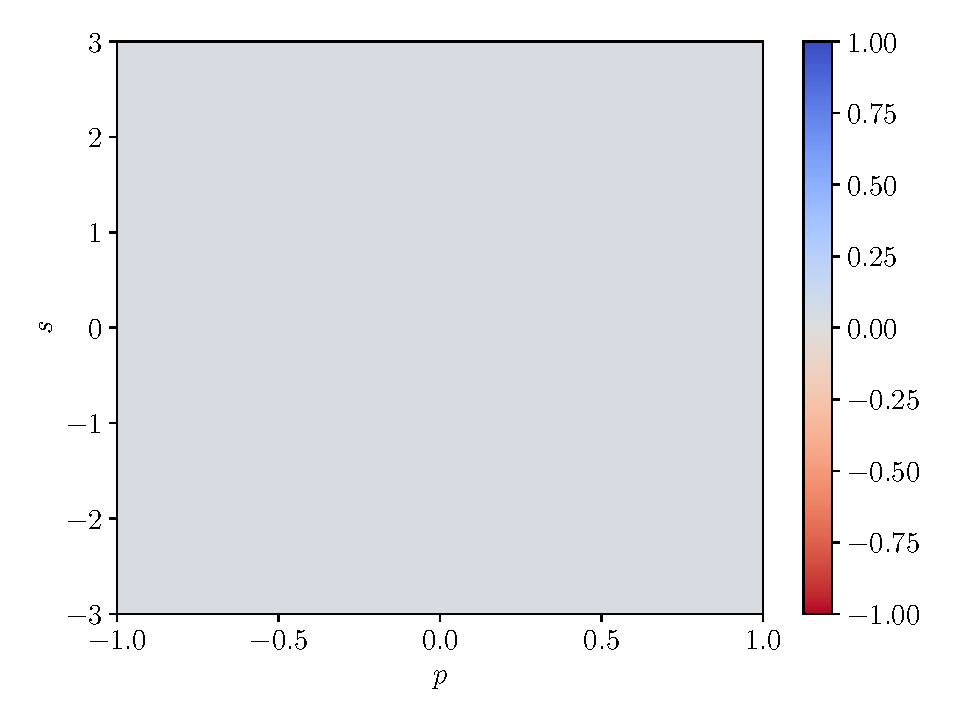
\includegraphics[width=\textwidth]{resources/pdf/2_dql_q0.pdf}
            \caption{$\hat{Q}(v(x), 0)$}
        \end{subfigure}
        \hfill
        \begin{subfigure}{0.49\textwidth}
            \centering
            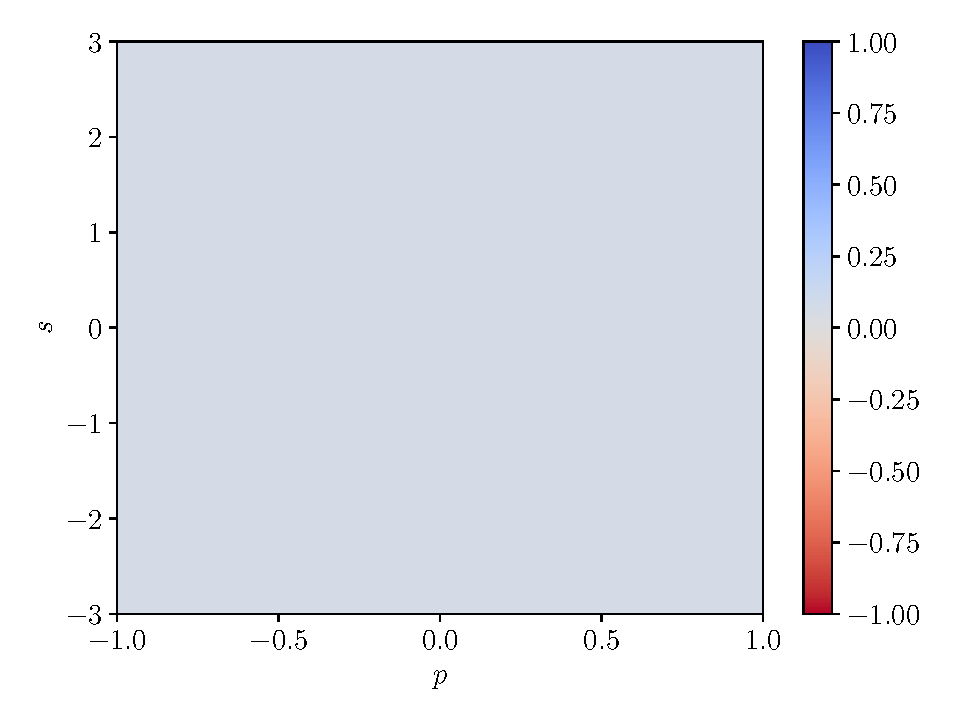
\includegraphics[width=\textwidth]{resources/pdf/2_dql_q1.pdf}
            \caption{$\hat{Q}(v(x), 1)$}
        \end{subfigure}
        \caption{$\hat{Q}$ values predicted by DQL.}
        \label{fig:dql.hat.q}
    \end{figure}
    
    We observe that the network predicts a null state-action value everywhere. This clearly means that it is unable to grasp the environment dynamics and, most importantly, the reward system.
    
    As one could expect, the expected return\footnotemark{} $J^{\hat{\mu}^*_N}$ of the policy inferred from $\hat{Q}$ 
    \begin{equation}\label{eq:mu.derived}
        \hat{\mu}^*(x) \in \arg\max_{u \in U} \hat{Q}(v(x), u)
    \end{equation}
    is null as well.
    
    \footnotetext{The expected return was estimated using the routines implemented for the previous assignment. The complete procedure is explained in the Appendix \ref{sec:expected.return}.}
    
    We repeated this experiment several times while modifying some hyper-parameters and the architecture, but it never worked out. Actually, this is not very surprising as it was mentioned during the course \cite{ernstinfo8003qfunctions} that it is very hard to perform regression on moving targets, which DQL implements. In fact, this is the main reason why a target network was introduced in \textcite{mnih2015human}. This will be covered in Section \ref{sec:dql.vs.dqn}.
    
    \section{Deep Q-Learning VS FQI-Trees}
    
    In this section, we compare our Deep Q-learning algorithm working with images as inputs with the algorithms implemented for the previous assignment.
    
    \subsection{FQI with XRT on images}
    
    Unfortunately, we were not able to implement Fitted-Q-Iteration (FQI) with Extremely Randomized Trees (XRT) for $v(x)$ inputs due to technical constraints. Indeed, (extremely) randomized trees is an offline estimator meaning that it requires to have the entire dataset stored in memory at once. Additionally, the number of nodes in randomized trees grows (linearly) with the number of estimators, the number of samples and (linearly) with the number of input features. Therefore, because the observations are $100 \times 100$ RGB images, we didn't manage to realize this experiment on our personal computers.
    
    Also, while searching for solutions, we noticed that there is a lack of literature around the topic of Randomized Trees applied to images. In fact, we were only able to find a few (rather old) relevant publications: \textcite{ernst2006reinforcement}, \textcite{bosch2007image}, \textcite{maree2007random}. This could indicate that such methods are not appropriate for this task, and therefore would have performed poorly. Although, it is very unlikely that it would have performed worse than the network of Section \ref{sec:dql}.
    
    \subsection{FQI with XRT and Parametric Q-learning with direct access to $x$}
    
    Conversely to the previous section, here, the estimators have direct access to the state $x$. In fact, this corresponds to the experiments we realized in the previous assignment. Therefore, instead of re-implementing the experiments, we simply re-use the results and plots of the previous report.
    
    It should be noted that we only kept the results with the \enquote{Monte Carlo} dataset generation strategy, \ie{} joining trajectories. Also, for FQI with XRT we selected the first stopping rule, \ie{} stop when $N=162$. Finally, for the parametric Q-learning (PQL), we used the Adam optimizer instead of regular SGD as the latter didn't produce relevant results. The results are presented in Figures \ref{fig:fqi.xrt} and \ref{fig:q.learning.nn.adam}.
    
    \begin{figure}[h]
        \centering
        \begin{subfigure}{0.49\textwidth}
            \centering
            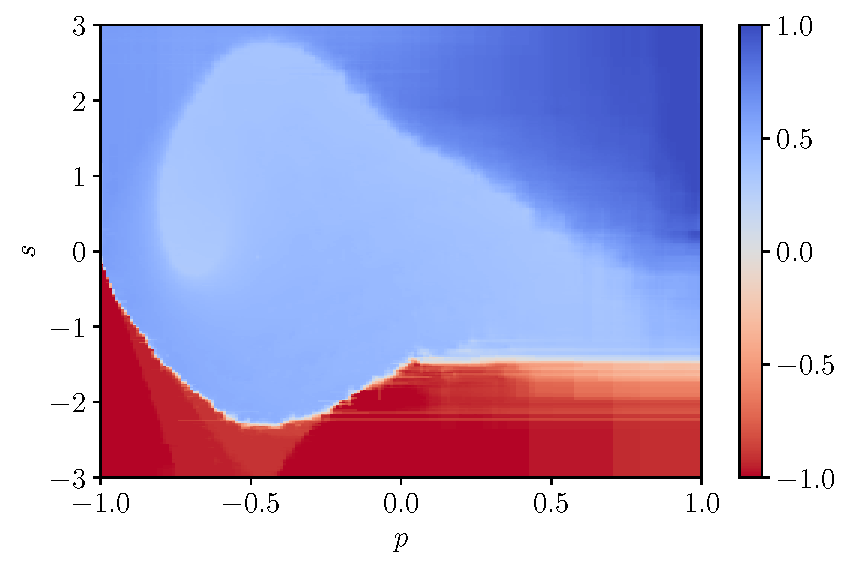
\includegraphics[width=\textwidth]{resources/pdf/previous_montecarlo_1_XRT_q0.pdf}
            \caption{$\hat{Q}_N(x, 0)$}
        \end{subfigure}
        \hfill
        \begin{subfigure}{0.49\textwidth}
            \centering
            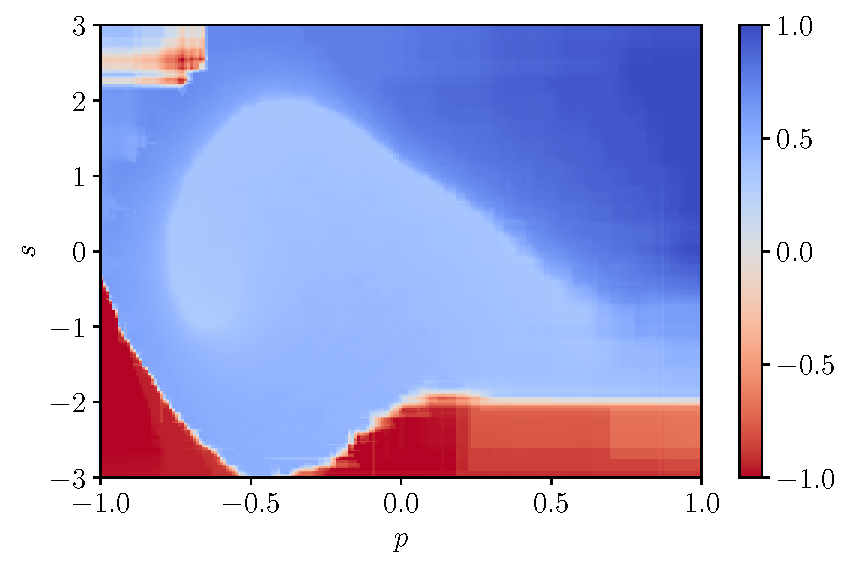
\includegraphics[width=\textwidth]{resources/pdf/previous_montecarlo_1_XRT_q1.pdf}
            \caption{$\hat{Q}_N(x, 1)$}
        \end{subfigure}
        \caption{$\hat{Q}_N$ values predicted by FQI with XRT; $N = 162$.}
        \label{fig:fqi.xrt}
    \end{figure}
    
    \begin{figure}[h]
        \centering
        \begin{subfigure}{0.49\textwidth}
            \centering
            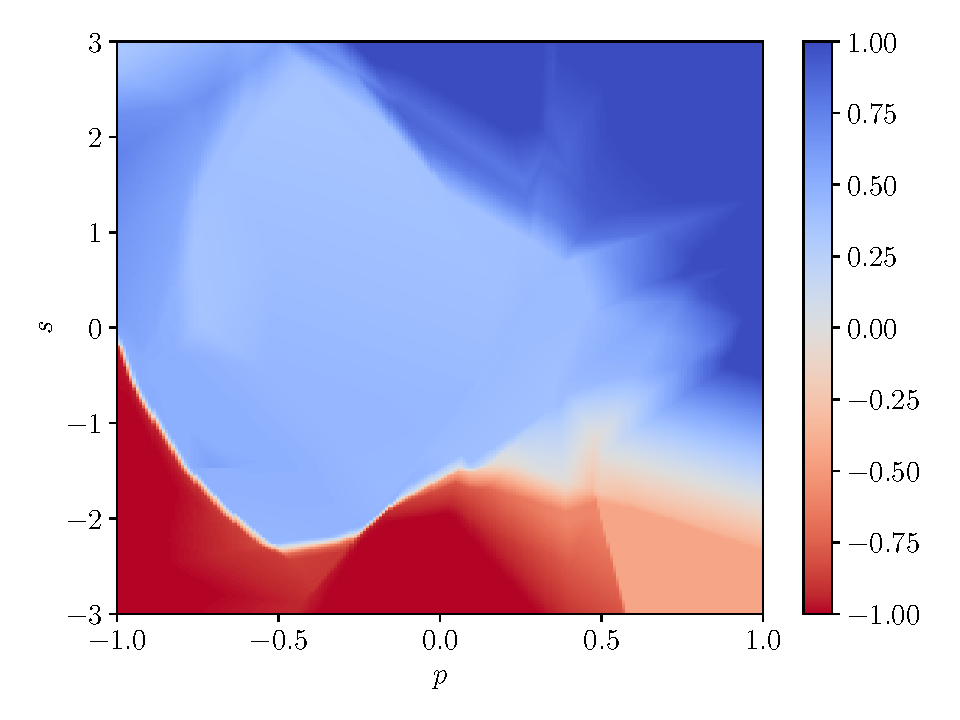
\includegraphics[width=\textwidth]{resources/pdf/previous_PQL_q0.pdf}
            \caption{$\hat{Q}(x, 0)$}
        \end{subfigure}
        \hfill
        \begin{subfigure}{0.49\textwidth}
            \centering
            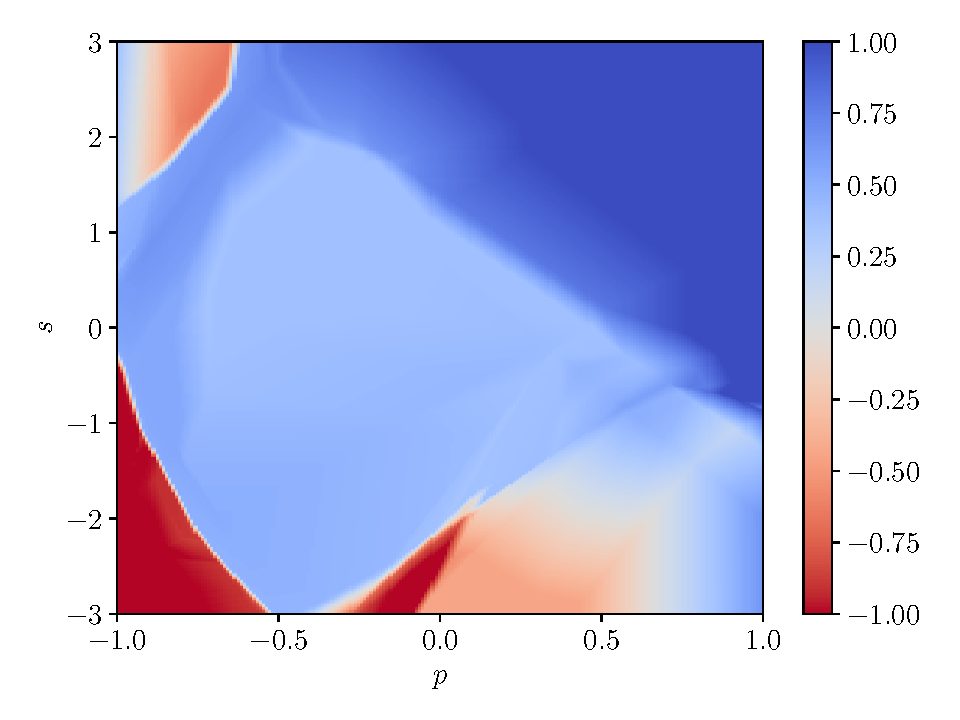
\includegraphics[width=\textwidth]{resources/pdf/previous_PQL_q1.pdf}
            \caption{$\hat{Q}(x, 1)$}
        \end{subfigure}
        \caption{$\hat{Q}$ values predicted by PQL.}
        \label{fig:q.learning.nn.adam}
    \end{figure}
    
    Concerning the expected returns of the inferred policies, FQI with XRT reached \num{0.42} while PQL reached \num{0.37}. These scores demonstrate a good understanding of the environment dynamics and reward system. But, it is not surprising that these methods perform much better than DQL on observations, as they have access to the \enquote{true} states. In Section \ref{sec:dql}, the network not only has to understand that its actions have an effect on the position and speed of the car, but also that there is a car and that it moves. Hence, the problem is inherently harder.
    
    However, the problem could have been even harder if the provided observations were too noisy or not enough informative to derive with certainty the internal state of the environment. This is the problem of \emph{acting under uncertainty} \cite{mccallum1997reinforcement}.
    
    \section{Deep Q-Learning VS Deep Q-Network} \label{sec:dql.vs.dqn}
    
    In this section, we compare our implementation of the \emph{Deep Q-learning} algorithm with the \emph{Double Q-learning} \cite{hasselt2010double, ernstinfo8003qfunctions} algorithm popularized by \textcite{mnih2015human}.
    
    Double Q-learning is exactly the same as Deep Q-learning, with the exception that it introduces a second neural network, called the \emph{target network}, that replaces the first network when computing the targets in the Q-learning updates. In practice, this target network is a clone of the main network and is updated periodically with the new weights of the latter. In their paper, \textcite{mnih2015human} explain that
    
    \begin{quote}
        \enquote{This modification makes the algorithm more stable compared to standard online Q-learning, where an update that increases $\hat{Q}(x, u)$ often also increases $\hat{Q}(x', u')$ for all $u'$ and hence also increases the target $r + \gamma \max_{u'} \hat{Q}(x', u')$, possibly leading to oscillations or divergence of the policy. Generating the targets using an older set of parameters adds a delay between the time an update to $\hat{Q}$ is made and the time the update affects the targets, making divergence of oscillations much more unlikely.}
    \end{quote}
    
    For our implementation of Double Q-learning, we keep the same network architecture and the same training routine as in Section \ref{sec:dql}, but we clone the main network at the beginning of each epoch to produce a target network.
    
    \subsection{Results}
    
    The state-action values, for each action, obtained using Double Q-Learning are shown in Figure \ref{fig:dqn.hat.q}.
    
    \begin{figure}[h]
        \centering
        \begin{subfigure}{0.49\textwidth}
            \centering
            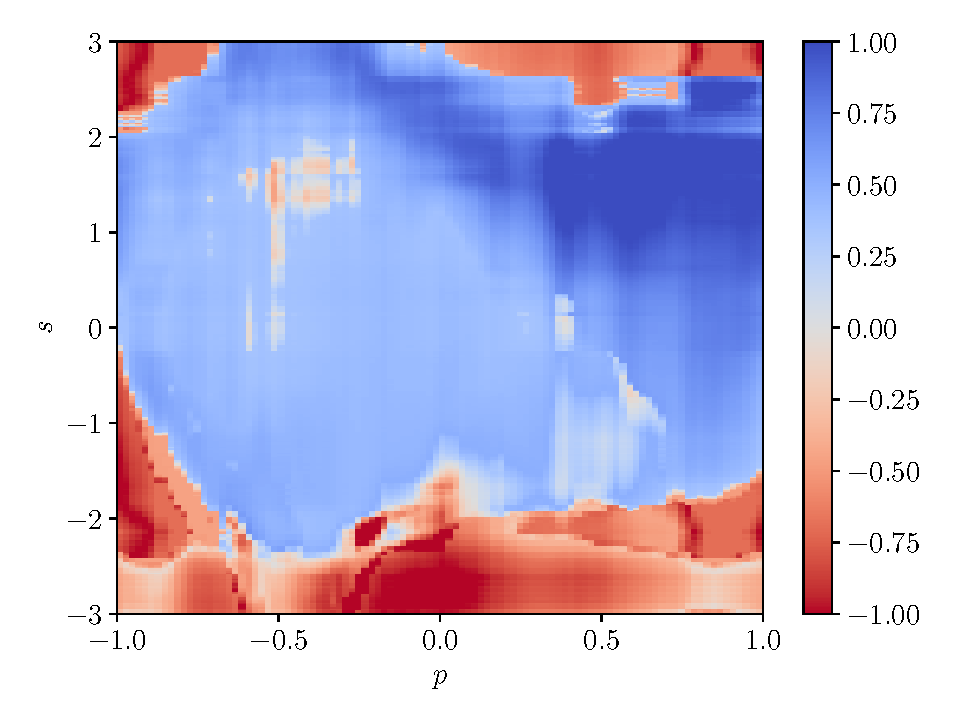
\includegraphics[width=\textwidth]{resources/pdf/4_dqn_q0.pdf}
            \caption{$\hat{Q}(v(x), 0)$}
        \end{subfigure}
        \hfill
        \begin{subfigure}{0.49\textwidth}
            \centering
            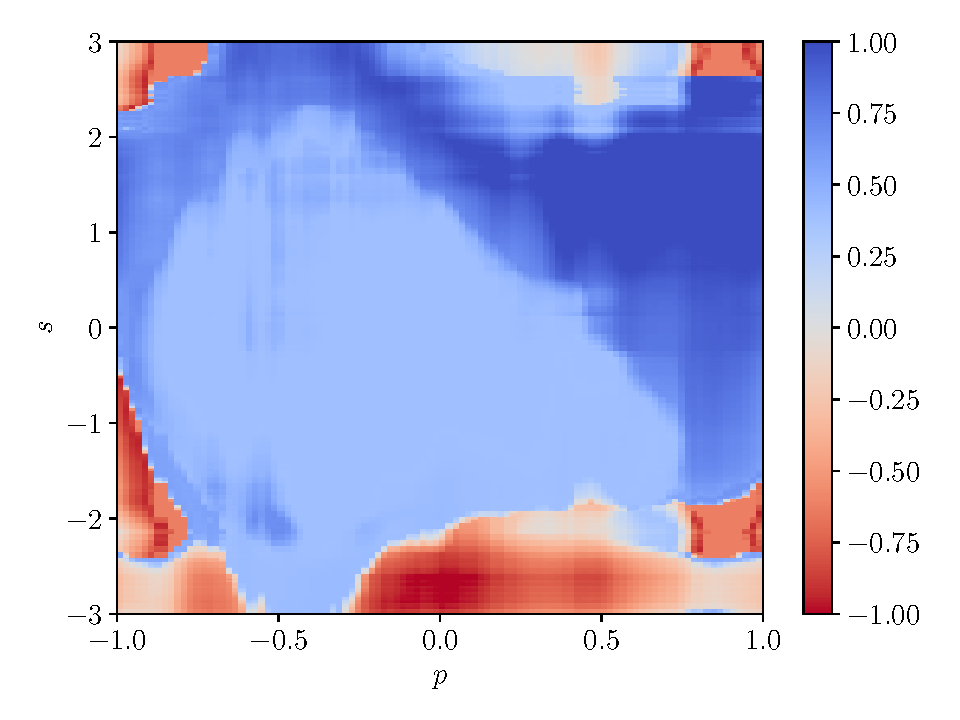
\includegraphics[width=\textwidth]{resources/pdf/4_dqn_q1.pdf}
            \caption{$\hat{Q}(v(x), 1)$}
        \end{subfigure}
        \caption{$Q$-values predicted by Double-QL.}
        \label{fig:dqn.hat.q}
    \end{figure}
    
    This time, the network seems to have understood fairly well the environment dynamics as the values of $\hat{Q}$ are quite close to those of FQI with XRT or PQL (\cf{} Figures \ref{fig:fqi.xrt} and \ref{fig:q.learning.nn.adam}). We do note, however, that the predictions are less \enquote{smooth} than those of FQI (or PQL) and present steep variations in some locations. Most importantly, Double Q-learning did a much better job than standard Deep Q-learning. Especially, the expected reward of the inferred policy reaches \num{0.38}, \ie{} barely worse than FQI (with XRT) and a bit better than PQL, while having only access to observations $v(x)$.
    
    \newpage
    
    \appendix
    
    \section{Expected Return of a Policy in Continuous Domain}\label{sec:expected.return}
    
    \begin{note}
        This section is a copy of the corresponding section in our previous assignment.
    \end{note}
    
    In the car-on-the-hill problem, the dynamics $f$ and reward signal $r$ of the environment are deterministic, \ie{} a state-action pair $(x, u)$ will always lead to the same one-step transition $(x, u, r, x')$. However, the choice of the initial state $x_0$ is stochastic. Therefore, the expected return $J^\mu$ of a policy $\mu$ can be expressed as
    \begin{equation}
        J^\mu = E_{x_0 \sim p(x_0)} \cbk{ \lim_{N \to \infty} \sum_{i = 0}^{N - 1} \gamma^i r(x_i, \mu(x_i)) }
    \end{equation}
    where $x_{i + 1} = f(x_i, \mu(x_i))$ and $\gamma \in [0; 1)$ is the discount factor. Interestingly, because $r$ is non-null only once in a trajectory, we have
    \begin{equation}
        \norm{J^\mu}_\infty \leq \norm{r}_\infty = B_r = 1 .
    \end{equation}
    In order to estimate the expected return, we have to fix a time horizon $N$ such that
    \begin{equation}\label{eq:N-expected.return}
        J^\mu_N = E_{x_0 \sim p(x_0)} \cbk{ \sum_{i = 0}^{N - 1} \gamma^i r(x_i, \mu(x_i)) }
    \end{equation}
    is a good approximation of $J^\mu$. In the car-on-the-hill environment, it can be shown \cite{ernstinfo8003, rozet2021suboptimality} that
    \begin{equation}
        \norm{J^\mu - J^\mu_N}_\infty \leq \gamma^N \norm{J^\mu} \leq \gamma^N B_r
    \end{equation}
    which can be used to enforce a certain precision. With a threshold $\epsilon = \num{e-2}$, we have
    \begin{align*}
        \gamma^N B_r & \leq \epsilon \\
        N & \geq \log_\gamma \frac{\epsilon}{B_r}
    \end{align*}
    which leads the smallest acceptable value
    \begin{equation} \label{eq:N-smallest.acceptable}
        N = \left\lceil \log_\gamma \frac{\epsilon}{B_r} \right\rceil = 90.
    \end{equation}
    Still, it is not possible to compute $J^\mu_N$ exactly as there is an infinite number of possible initial states $x_0$. Therefore, the expectation has to be approximated as well. This is done using the \emph{Monte Carlo} method, \ie{} approximating the expected return by the average cumulative reward over several trajectories. Let $h = (x_0, u_0, r_0, x_1, \dots, u_{t - 1}, r_{t - 1}, x_t)$ denote a trajectory of length $t$. Since $x_t$ can be the only terminal state of $h$, the cumulative reward $C_h$ is computed as
    \begin{equation}
        C_h = \sum_{i = 0}^{t - 1} \gamma^i r_i = \gamma^{t - 1} r_{t - 1} .
    \end{equation}
    Then, to estimate $J^\mu_N$, we simulate $n$ trajectories $h_i$ of length $N$ or less and compute
    \begin{equation}
        J^\mu_N \simeq \frac{1}{n} \sum_{i = 0}^{n - 1} C_{h_i} .
    \end{equation}
    
    \newpage

    \printbibliography
\end{document}
